\loai{Dây dẫn uốn 1 phần thành vòng tròn}
\begin{vidu} %[2P4-3.3K][Loại1]
immini[thm]{Một dây dẫn thẳng dài có đoạn giữa uốn thành hình vòng tròn như hình vẽ. Cho dòng điện chạy qua dây dẫn theo chiều mũi tên thì vector cảm ứng từ tại tâm O của vòng tròn có hướng
\choice
{thẳng đứng hướng lên trên}
{vuông góc với mặt phẳng hình tròn, hướng ra phía sau}
{\True vuông góc với mặt phẳng hình tròn, hướng ra phía trước}
{thẳng đứng hướng xuống dưới}}{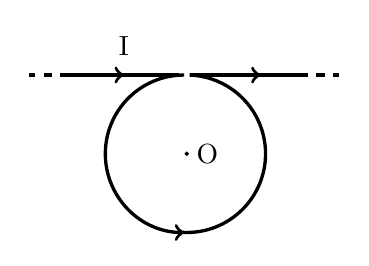
\begin{tikzpicture}
\coordinate (a) at (0,0);
\draw [very thick,->](a)--++(0:0.7)node[above=3pt]{\normalsize{\bth{I}}};
\draw [very thick](a)--++(0:1.4)coordinate (c);
\draw [very thick,dashed](a)--++(180:0.5);
\path (c) ++(270:1)++(0:0.1)coordinate (o);
\filldraw[black] (o) circle(0.02)node[right]{\normalsize{\bth{O}}};
\draw [very thick,->](o)++(92:1) arc (90:270:1) ;
\draw [very thick](o)++(265:1) arc (265:448:1) coordinate (d);
\draw [very thick,->](d)--++(0:0.9);
\draw [very thick](d)--++(0:1.4)coordinate (e);
\draw [very thick,dashed](e)--++(0:0.5);
\end{tikzpicture}}
\loigiai{\begin{itemize}
\item Áp dụng quy tắc bàn tay phải ta thấy vector $\vec{B}_1$ hướng vào trong; $\vec{B}_2$ hướng ra phía trước, độ lớn của $B_2$ do phần dòng điện tròn gây ra lớn hơn.
\item Vậy $B=|B_1-B_2|$ vuông góc với mặt phẳng hình tròn, hướng ra phía trước.
\end{itemize}
}
\end{vidu}
\begin{vidu} %[2P4-3.3K][Loại1]
immini[thm]{Một dây dẫn rất dài được căng thẳng trừ một đoạn ở giữa dây uốn thành một vòng tròn bán kính 1,5 cm. Cho dòng điện 3 A chạy trong dây dẫn. Xác định cảm ứng từ tại tâm của vòng tròn nếu vòng tròn và phần dây thẳng cùng nằm trong một mặt phẳng}{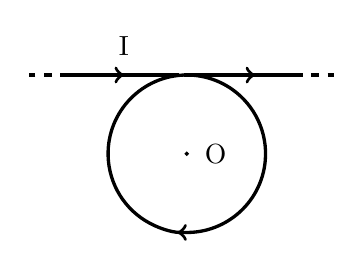
\begin{tikzpicture}
\coordinate (a) at (0,0);
\draw [very thick,->](a)--++(0:0.7)node[above=3pt]{\normalsize{\bth{I}}};
\draw [very thick](a)--++(0:1.4)coordinate (c);
\draw [very thick,dashed](a)--++(180:0.5);
\path (c) ++(270:1)++(0:0.1)coordinate (o);
\filldraw[black] (o) circle(0.02)node[right=3pt]{\normalsize{\bth{O}}};
\draw [very thick,-<](o)++(88:1) arc (88:270:1) ;
\draw [very thick](o)++(265:1) arc (265:452:1) coordinate (d);
\draw [very thick,->](d)--++(0:0.9);
\draw [very thick](d)--++(0:1.4)coordinate (e);
\draw [very thick,dashed](e)--++(0:0.5);
\end{tikzpicture}}
\choice
{$5,6.10^{-5}\ T$}
{$6,6.10^{-5}\ T$}
{$7,6.10^{-5}\ T$}
{\True $16,6.10^{-5}\ T$}
\loigiai{\begin{itemize}
\item Cảm ứng từ do các dòng điện gây ra tại tâm O:
\begin{align*}
\begin{cases}
	B_1=2\pi.10^{-7}.\dfrac{I}{R}\\
	B_2=2 .10^{-7}.\dfrac{I}{R}
\end{cases}
\end{align*}
\item Do $\vec{B}_1\ \text{cùng chiều}\ \vec{B}_2 \Rightarrow B=B_1+B_2 = 2.10^{-7}.\dfrac{I}{R}.(\pi+1)=1,7.10^{-5}$ T.
\end{itemize}}
\end{vidu}
\loai{Hai dòng điện tròn đồng tâm, nằm trong cùng 1 mặt phẳng}
\begin{vidu} %[2P4-3.3K][Loại2]
Hai vòng tròn dây dẫn đồng tâm, bán kính một vòng là $R_1 = 8$ cm, vòng kia là $R_2 = 16$ cm, trong mỗi vòng dây đều có dòng điện cường độ $I = 10$ A chạy qua. Biết hai vòng dây nằm trong cùng một mặt phẳng, và dòng điện chạy trong hai vòng ngược chiều. Cảm ứng từ tại tâm của hai dây dẫn có độ lớn là
\choice
{$1,18.10^{-4}$ T}
{$1,2.10^{-4}$ T}
{\True $3,9.10^{-5}$ T}
{$8,8.10^{-5}$ T}
\loigiai{Do hai dòng điện tròn đồng tâm, ngược chiều, cùng nằm trên một mặt phẳng, do đó $\vec{B}_1$ và $\vec{B}_2$ do hai dòng điện tròn gây ra tại tâm ngược chiều.
$B = |B_1 - B_2| = 3,9.10^{-5}$ T}
\end{vidu}
\loai{Hai dòng điện tròn đồng tâm, nằm trong 2 mặt phẳng vuông góc}
\begin{vidu} %[2P4-3.3K][Loại3]
Tính cảm ứng từ tại tâm của hai vòng tròn dây dẫn đồng tâm, bán kính một vòng là $R_1=8\ cm$, vòng kia là $R_2=16\ cm$, trong mỗi vòng dây đều có dòng điện cường độ $I=10\ A$ chạy qua. Biết hai vòng dây nằm trong hai mặt phẳng vuông góc với nhau.
\choice
{\True $8,8.10^{-5}\ T$}
{$7,6.10^{-5}\ T$}
{$6,8.10^{-5}\ T$}
{$3,9.10^{-5}\ T$}
\loigiai{\begin{itemize}
\item Cảm ứng từ do các dòng điện gây ra tại tâm O:
\begin{align*}
\begin{cases}
B_1=2\pi.10^{-7}.\dfrac{I}{R_1}=2,5\pi .10^{-5}\\
B_2=2\pi .10^{-7}.\dfrac{I}{R_2}=1,25\pi .10^{-5}
\end{cases}
\end{align*}
\item Do $\vec{B}_1 \perp \vec{B}_2 \Rightarrow B=\sqrt{B_1^2+B_2^2} \approx 8,8.10^{-5}$ T.
\end{itemize}}
\end{vidu}
\loai{Từ trường tổng hợp của dòng điện tròn với từ trường ngoài}
\begin{vidu} %[2P4-3.3K][Loại4]
Một vòng dây hình tròn, bán kính $R=10$ cm có dòng điện $I=10$ A chạy qua, được đặt song song với đường cảm ứng từ của một từ trường đều có cảm ứng từ $B_0=8.10^{-5}\ T$. Xác định góc giữa cảm ứng từ tổng hợp tại tâm O của vòng dây đó và $\vec B_0$.
\choice
{$28^\circ 40'$}
{$18^\circ 10'$}
{$58^\circ 20'$}
{\True $38^\circ 10'$}
\loigiai{
immini[thm]{Vector cảm ứng từ $\vec{B}_1 $ do vòng dây mang dòng điện I gây ra tại tâm O có phương vuông góc với mặt phẳng vòng dây, có chiều theo quy tắc đinh ốc và có độ lớn: $B_1=2\pi.10^{-7}.\dfrac{I}{R}=6,3.10^{-5}\ T.$
\begin{itemize}
\item Cảm ứng từ tổng hợp tại O như hình vẽ: $\vec{B}=\vec{B}_1+\vec{B}_0$.
\item Và có độ lớn (vì $\vec{B}_1\bot \vec{B_0} $): $B=\sqrt{B^2_1+B^2_0}\approx 1,0.10^{-4}\ T $; có phương lập với $\vec{B_0} $ một góc $\alpha $ mà $\tan \alpha =\dfrac{B_1}{B_0}=7,8 \Rightarrow \alpha =38^\circ10'$ .
\end{itemize}}{\begin{tikzpicture}
\draw[undirected](0,0) arc (20:-160:2 and 1);
\draw[directed](0,0) arc (20:200:2 and 1);
\draw[->] (-2,0)coordinate(o)--(1,0)coordinate(b0)node[right]{$\vec{B}_0$};
\draw[->] (-2,0)--(-2,2)node[left]{$\vec{B}_1$};
\draw[->] (-2,0)--(1,2)coordinate(b)node[right]{$\vec{B}$};
\draw[dashed] (-2,2)--(1,2)--(1,0);
\tkzMarkAngles[size=0.5cm](b0,o,b)
\tkzLabelAngles[pos=0.8](b0,o,b){$\alpha$}
\end{tikzpicture}}}
\end{vidu}
\loai{Cảm ứng từ trong lòng ống dây đặt trong từ trường trái đất}
\begin{vidu} %[2P4-3.3G][Loại5]
immini[thm]{Một vòng dây dẫn tròn bán kính $R=5$ cm, có dòng điện $I=1,6$ A đi qua, đặt nằm ngang song song với từ trường $\vec{B}_0 $ của Trái đất có độ lớn $B_0=2.10^{-5}\ T$. Tìm góc quay của kim nam châm nhỏ đặt tại tâm vòng dây khi ngắt dòng điện I.
\choice
{$30^\circ$}
{\True $45^\circ$}
{$60^\circ$}
{$75^\circ$}
}
{\begin{tikzpicture}[scale=1,thick,>=stealth',rotate=-90]
		\draw[undirected](0,0) arc (0:-180:1 and 2.5);
		\draw[directed](0,0) arc (0:180:1 and 2.5);
		\draw[->] (-1,0)--(-1,2)coordinate(b0)node[below left]{$\vec{B}_0$};
\end{tikzpicture}}
\loigiai{
immini[thm]{\begin{itemize}
\item Tìm $\vec{B} =\vec{B_0}+\vec{B}_1 $ (với $\vec{B}_1$ là véctơ cảm ứng từ do vòng dây ra tại tâm vòng dây).
\item Ta thấy góc giữa $\vec{B} $ và $\vec{B_0} $ là góc $\alpha$ với $\tan \alpha =\dfrac{B_1}{B_0}\approx 1 \rightarrow \alpha =45^\circ $.
\item Khi chưa ngắt dòng điện, kim nam châm hướng theo $\vec{B} $.
\item Khi ngắt dòng điện (không có $\vec{B}_1 $), kim nam châm hướng theo $\vec{B_0} $.
\item Như vậy khi ngắt dòng điện, kim nam châm quay một góc bằng $\alpha=45^\circ$.
\end{itemize}}
{
\begin{tikzpicture}[scale=1,thick,>=stealth']
\draw[undirected](0,0) arc (0:-180:1 and 2.5);
\draw[directed](0,0) arc (0:180:1 and 2.5);
\draw[->] (-1,0)coordinate(o)--(1,0)node[right]{$\vec{B}_1$};
\draw[->] (-1,0)--(-1,2)coordinate(b0)node[below left]{$\vec{B}_0$};
\draw[->] (-1,0)--(1,2)coordinate(b)node[right]{$\vec{B}$};
\draw[dashed] (-1,2)--(1,2)--(1,0);
\tkzMarkAngles[size=0.4cm](b,o,b0)
\tkzLabelAngles[pos=0.7](b,o,b0){$\alpha$}
\end{tikzpicture}
}
}
\end{vidu}
